	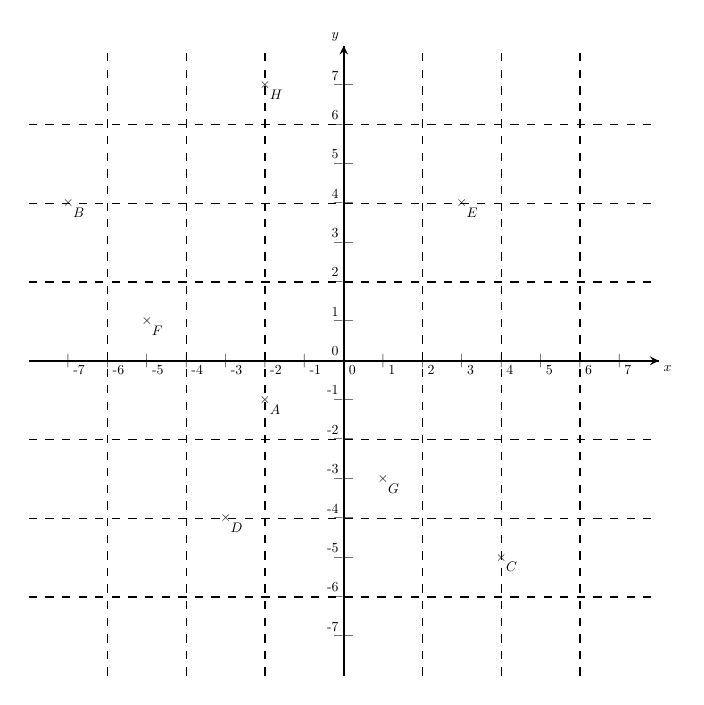
\begin{tikzpicture}[scale=0.5,every node/.style={scale=0.5}]
		%Points
		\coordinate(O)at(0,0);
		\coordinate(I)at(1,0);
		\coordinate(J)at(0,1);
		\coordinate(xstart)at(-8,0);
		\coordinate(xend)at(8,0);
		\coordinate(ystart)at(0,-8);
		\coordinate(yend)at(0,8);
		\coordinate(A)at(-2,-1);
		\coordinate(B)at(-7,4);
		\coordinate(C)at(4,-5);
		\coordinate(D)at(-3,-4);
		\coordinate(E)at(3,4);
		\coordinate(F)at(-5,1);
		\coordinate(G)at(1,-3);
		\coordinate(H)at(-2,7);
		%Étiquettes
	%	\draw (I) node[below right] {$1$};
	%	\draw (J) node[above left] {$1$};
		\draw (xend) node[below right] {$x$};
		\draw (yend) node[above left] {$y$};	
		%%%%%%%%%%%%%%%%%%%%%%%%%%%%%%%%%%%%
		%Axes
		\draw [thick] (xstart) -- (xend);
		\draw [thick] (ystart) -- (yend);
		%Flèches
	%	\draw [>=stealth,->] (O) -- (I);
	%	\draw [>=stealth,->] (O) -- (J);
		\draw [>=stealth,->] (O) -- (xend);
		\draw [>=stealth,->] (O) -- (yend);
	%	%Grille
	%	\draw [thin] (-8,-8)grid(8,8);
		%%%%%%%%%%%%%%%%%%%%%%%%%%%%%%%%%%%%
		%étiquettes
		\foreach \point in {A, ..., H}
			\draw(\point)node{$\times$};
		\foreach \point in {A, ..., H}
			\draw(\point)node[below right]{$\point$};		
		\foreach \r in {-7, -6, ..., 7}
	    	\draw[thick, below right] (\r,0) node{\r};
		\foreach \r in {-7, -6, ..., 7}
	    	\draw[thick, above left] (0,\r) node{\r};  
		\foreach \r in {-7, -6, ..., 7}
	    	\draw[thick] (\r,0) node{$|$};
		\foreach \r in {-7, -6, ..., 7}
	    	\draw[thick] (0,\r) node{$--$};
	   	\foreach \r in {-6, -4, ..., 6}
	    	\draw[dashed] (-8,\r)--(8,\r);
	   	\foreach \r in {-6, -4, ..., 6}
	    	\draw[dashed] (\r,-8)--(\r,8);
	%	\foreach \r in {0, 1,...,7}
	%    	\draw[thick, below right] (\r,0) node{\r};
	\end{tikzpicture}
